\section{Evaluation} \label{eval}

We implemented Tempus in $\sim600$ lines of Julia \cite{julia} code.
This code will take a topology configuration, source and destination node, and the 
temporal property in question and its threshold.
It will then output the final probability of the network upholding that temporal property.
We ran our prototype on a machine with 2 Intel E5-2630 v3 8-core CPU running up to 2.4 GHz 
and 128 GB of ECC RAM, provided by CloudLab \cite{cloudlab}.

To appraise the viability of our approach, we seek to answer 5 evaluation questions:
\begin{enumerate}
    \item How long does it take to run the verifier overall? How does it scale?
    \item What is the bottleneck step in the verification process?
    \item How effective is the optimization technique in reducing the verification time?
    \item How effective is the optimization technique in reducing the explored equivalence classes?
    \item How does different topologies affect optimization effectiveness?
\end{enumerate}

\subsection{Experiment Setup}

\begin{table}[h]
    \begin{tabular}{| c | c | c | c |}
    \hline
    Topology & \#routers & \#links & type \\
    \hline
    Fat Tree 4 & 20 & 32 & DC \\
    Fat Tree 6 & 45 & 108 & DC \\
    Fat Tree 8 & 80 & 256 & DC \\
    Fat Tree 10 & 125 & 500 & DC \\
    Fat Tree 12 & 180 & 864 & DC \\
    Fat Tree 14 & 245 & 1372 & DC \\
    Fat Tree 16 & 320 & 2048 & DC \\
    Fat Tree 24 & 720 & 6912 & DC \\
    Fat Tree 32 & 1280 & 16384 & DC \\
    Latnet & 69 & 74 & WAN \\
    Highwinds & 18 & 31 & WAN \\
    AT\&T & 25 & 56 & WAN \\
    Uninett & 74 & 101 & WAN \\
    GtsCe & 149 & 193 & WAN \\
    \hline
\end{tabular}
\caption{List of topologies being tested}
\label{tab:topologies}
\end{table}

We tested Tempus on 5 real-world WAN topologies from the Topology Zoo and 3 datacenter topologies 
(fat-tree, with various amount of pods).
%TODO: stats of the topologies

\subsubsection{Functional Verification}
As verifying the routing protocol functional behavior is not the primary contribution of our research, 
we simply use OSPF as the routing protocol in our experiment with uniform link weights of 1.
We set 0.1\% failure rate in all links, in accordance to the failure rate in previous studies. %TODO: cite
We then run the functional verification with $10^{-8}$ inaccuracy level.

In order for our evaluation to be realistic, we set the source and destination node to be one of the 
edge routers (node with the smallest degree / smallest centrality?).
%TODO: edge-to-edge routers

\subsubsection{Temporal Verification}
For latency distribution, we show that we can use an empirical measurement as a distribution by 
using the reported queue length from DCTCP \cite{dctcp}.
By multiplying the queue length distribution with the line-rate, we could approximate the queuing 
latency distribution for a given router. 

Since the CDF operation that we define for temporal property verification is relatively cheap, 
we expect our result to generalize with any threshold we chose. 
In other words, while changing the threshold will change the final probability, it won't change 
the runtime performance of Tempus.
Thus, we set an arbitrary threshold for our evaluation.

\subsection{Runtime Profiling}

\begin{figure}[h]
    \centering
    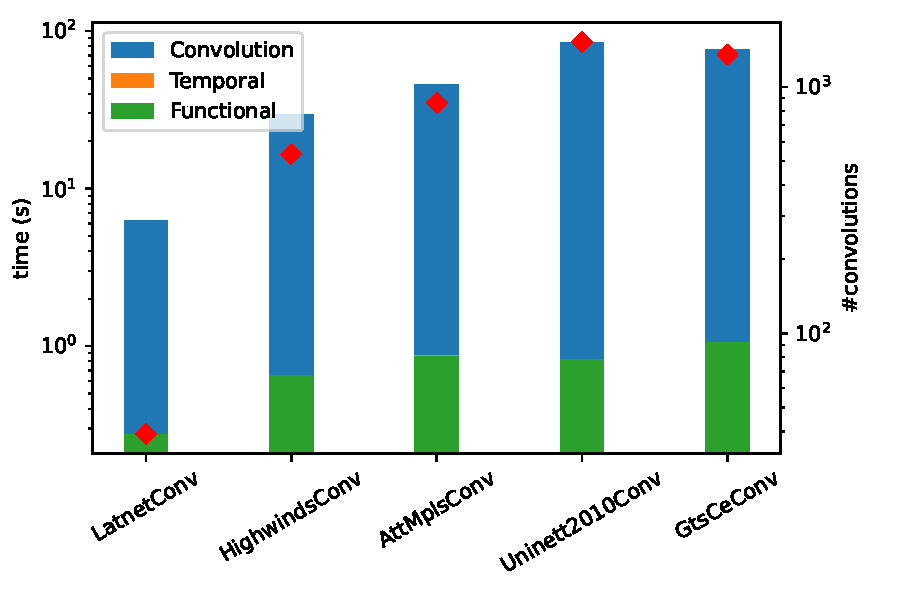
\includegraphics[scale=0.5]{scalability}
    \caption{Runtime performance of the verification process, red dots represent the number of convolutions}
    \label{fig:scalability}
\end{figure}

\begin{figure}[h]
    \centering
    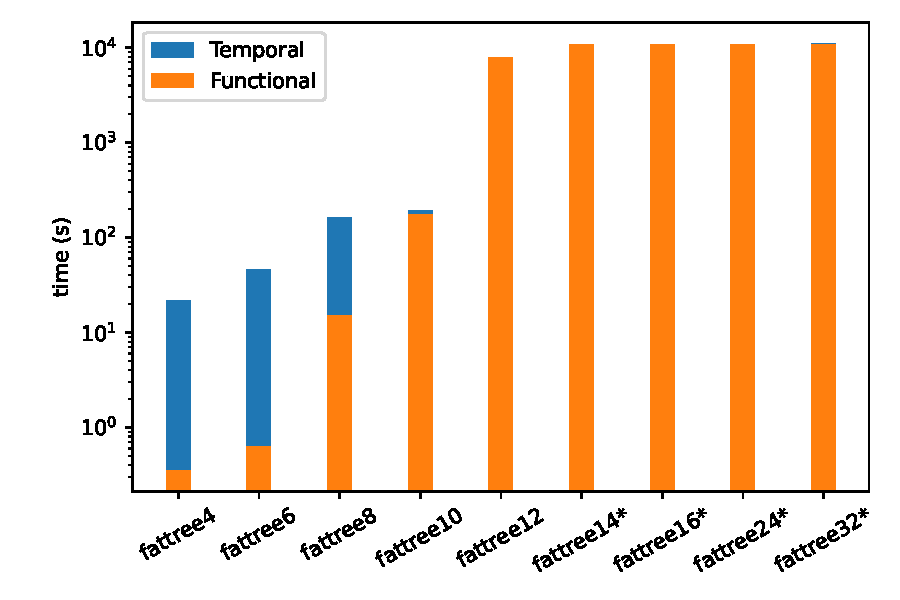
\includegraphics[scale=0.5]{scalability_fattree}
    \caption{Fat Tree, red dots represent the number of convolutions}
    \label{fig:scalabilityfat}
\end{figure}

\subsubsection{Performance and Scalability}
To begin our evaluation, we first measured the running duration of the verification process (and its steps) 
on various topologies.
Our results in Fig. \ref{fig:scalability} shows that our verification technique finished within a reasonable timeframe.
The verifier finished in the order of minutes, even for topologies with hundred of nodes.

From the same result, we also note that our verifier scales gracefully over the size of the network.
The verification duration ranges from 6 seconds to around 15 minutes. 
% TODO: fat-tree scalability
To drive this point more precisely, we also evaluate the running time of fat-tree topology in various sizes.
Our results in Fig. \ref{fig:scalabilityfat} shows that by keeping the same type of topology and scaling them up, we increased 
our verification time almost linearly, while the unoptimized version timed out after 2 hours.
Not only that, our combined optimization strategies actually reduces the time for fat tree topology of $k=10$ compared to 
equivalent topologies with smaller size.

\subsubsection{Bottleneck}
By looking at the proportion of time spent on each step in Fig. \ref{fig:scalability}, we could see that 
the combined \textbf{convolution procedure is the bottleneck} step in our verifier.
The convolution procedure takes 95\% - 99\% of the duration of the overall verification.
Hence we can see in the same figure that the runtime performance of Tempus and the total amount 
of convolution is highly correlated.

We conclude that for a reasonably low imprecision level, \textbf{Tempus runs in the order of 
minutes} and the performance of Tempus is primarily \textbf{bottlenecked by the total convolution 
operations}.

\subsection{Optimization Effectiveness}

\begin{figure}[h]
    \centering
    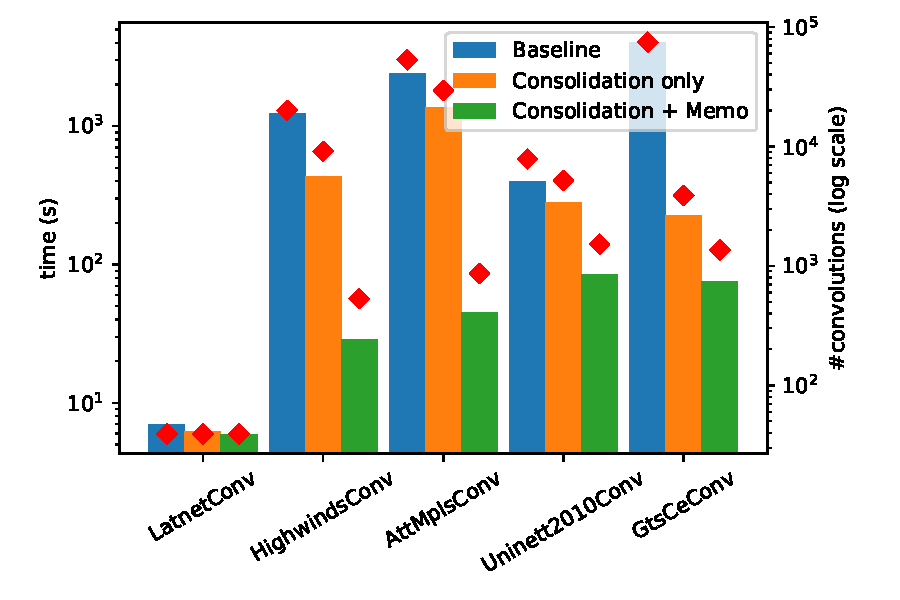
\includegraphics[scale=0.5]{optimization}
    \caption{Amount of convolution (in log scale) depending on what optimization strategy is applied}
    \label{fig:opt}
\end{figure}
\begin{figure}[h]
    \centering
    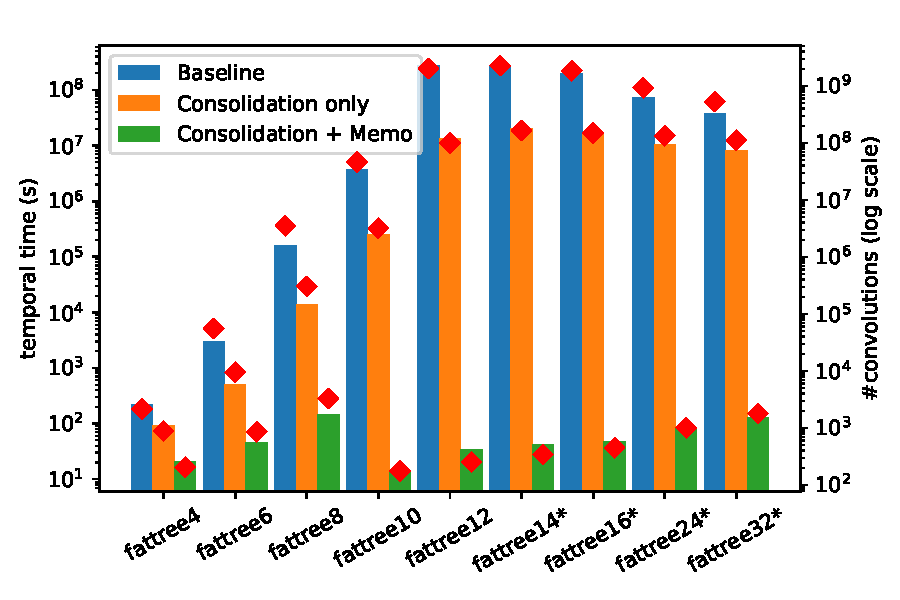
\includegraphics[scale=0.5]{optimization_fattree}
    \caption{Amount of convolution (in log scale) depending on what optimization strategy is applied}
    \label{fig:opt_fat}
\end{figure}

We have established that the convolution procedure is a relatively expensive operation within 
our verifier.
Next, we inspected the effectiveness of our optimization techniques in reducing them.
To do that, we measured the overall running duration of the verifier while selectively disabling the 
optimization.

Our results in Fig. \ref{fig:opt} shows the effect of the two optimization techniques we introduced -- 
consolidation and memoization -- in reducing the verification duration and amount of convolution (both in log scale).
For baseline, we ran the verifier without any optimization, resulting in the left bar.
The middle bar represents the result where we enable only the consolidation strategy.
Finally, the right bar represents the result where we enable both the consolidation and memoization strategy.

We note that for most of the topologies, the combination of both optimization strategies resulted in 
\textbf{79\% - 98\% improvement in performance}.
Compared to the baseline performance, the consolidation strategy contributes to 30\% - 94\% of the improvement and
the memoization strategy contributes to 67\% - 96\% on top of that. 
%TODO: factors of the network node-pair? path amount and length?

We conclude that \textbf{consolidation and memoization are both effective optimization strategies} in our verification
framework.

\subsection{Equivalence Class Reduction}

\begin{figure}[h]
    \centering
    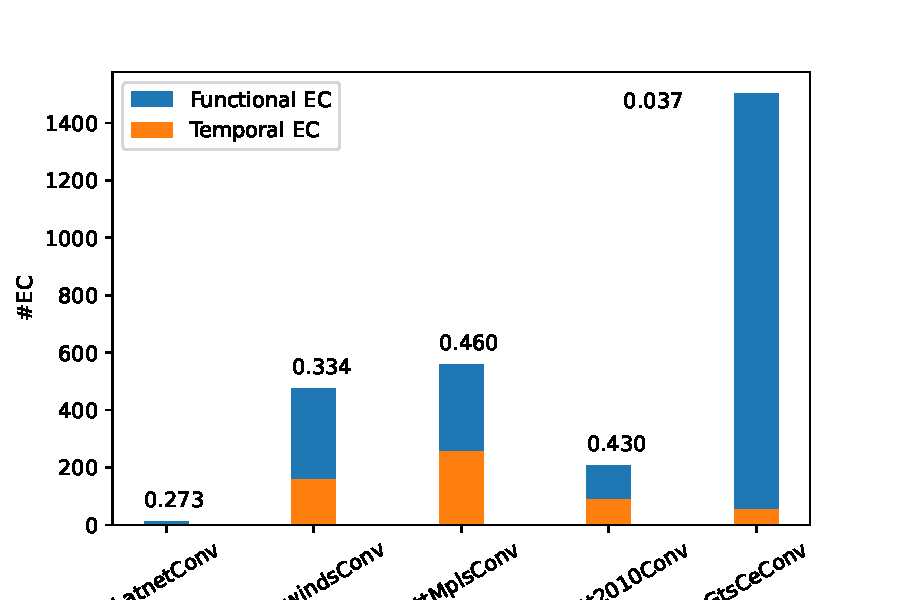
\includegraphics[scale=0.5]{ec}
    \caption{Amount of temporal EC compared to functional EC, label represents ratio}
    \label{fig:ec}
\end{figure}

While we cannot directly compare Tempus with other verifiers (due to difference in verification goal), 
we could use the amount of equivalence class as an indirect proxy of the verifier's behavior and performance.
Therefore, we measured the amount of additional equivalence classes introduced by Tempus in order to 
indirectly compare its overhead in addition to its functional counterparts.
This result is only influenced by the consolidation strategy, since the memoization strategy operates on 
a smaller granularity than equivalence classes.

Our results in Fig. \ref{fig:ec} shows the ratio between the amount of temporal equivalence classes that is 
being re-explored and the amount of functional equivalence class.
We note that we only need to \textbf{re-explore 4\% to 46\% equivalence classes} as an additional overhead 
compared to functional verification.

We conclude that \textbf{consolidation is effective in reducing the amount of equivalence classes that 
needs to be re-explored} in our verification framework.

\subsection{Optimization Analysis}

\begin{table}[h]
    \begin{tabular}{| c | c | c | c | c |}
        \hline
        Top. & \# path & \# path (cons) & \# path (base) & \# conv \\
        \hline
        % Latnet & 0\% & 4.2 \\
        % Highwinds & 97.7\% & 581.41  \\
        % AT\&T & 98.4\% & x \\
        % Uninett & 82.5\% & 108.87 \\
        % GtsCe & 98.2\% & 571.14 \\
        ft4 & 20 & 92 & 251 & 204 \\
        ft6 & 81 & 1,278 & 7,857 & 855 \\
        ft8 & 304 & 42,892 & 500,195 & 3280 \\
        ft10 & 25 & 456,700 & 6,669,169 & 175 \\
        ft12 & 36 & 14,367,491 & 288,537,289 & 252 \\
        ft14* & 49 & 23,767,482 & 323,686,008 & 343 \\
        ft16* & 64 & 21,272,060 & 261,254,848 & 448 \\
        ft24* & 144 & 19,064,581 & 132,197,345 & 1008 \\
        ft32* & 256 & 15,926,575 & 75,783,276 & 1792 \\
        \hline
    \end{tabular}
    \caption{Effectiveness metric}
    \label{tab:analysis}
\end{table}

Up to this point, we have demonstrated that consolidation and memoization are two effective strategies in 
reducing the verification duration and amount of convolution procedure that needs to be done.
However, the results also show that their effectiveness varies depending on the topology.

To examine the factors that affects the effectiveness of each optimization strategy, we compute some properties 
of the topology that relates to the nature of the optimization.

The effectiveness of the memoization strategy largely reflects the amount of unique paths that the functional 
verifier has explored.
The amount of unique paths (relative to the total explored paths) and the amount of reduction the memoization 
strategy gains is highly correlated, as shown by Tab. X

On the other hand, the effectiveness of the consolidation strategy is caused by more factors, such as the 
topology and the particular load-balancing scheme of the network protocol. 
As a proxy to this, we count the number of path that crosses each link, and averaged them.
As we could see from Tab. X, Uninett2010 has a measure of about 108.87, reflecting the relative ishortcoming 
of this particular strategy compared to another topology like GtsCe, which has a measure of 571.14.

% \begin{itemize}
%     \item While the amount of path in those states can explain the amount of EC reduction, to get to 
%         the amount of convolution, we also need to consider the length of each of those path
%     \item By considering the both amount of path and its length to counting the convolution, we could 
%         compare consolidation and memoization strategy to the unoptimized version
% \end{itemize}

% \begin{itemize}
%     \item Compare the amount of temporal EC to the functional (unconsolidated) EC
%     \item Corresponds to the consolidation strategy
%     \item \textbf{More than 50\% reduction}
%     \item Doesn't work equally on all topologies, depend on 
%     \begin{itemize}
%         \item How many functional EC are explored (for a given inaccuracy level)
%         \item How many possible paths a given node pair have in those ECs
%     \end{itemize}
% \end{itemize}